%% =========================================================
%% PRX main-manuscript draft focused on transient freezing
%% =========================================================

\documentclass[aps,prx,reprint,superscriptaddress,longbibliography,nofootinbib,floatfix]{revtex4-2}

\usepackage{graphicx}
\usepackage{dcolumn}
\usepackage{bm}
\usepackage{amsmath}
\usepackage{amssymb}
\usepackage{physics}
\usepackage{hyperref}
\hypersetup{
    colorlinks=true,
    linkcolor=blue,
    citecolor=blue,
    urlcolor=blue
}

\begin{document}

\title{Transient Freezing Governs Flat-Minimum Selection in Stochastic Gradient Descent}

\author{Ning Yang}
\thanks{These authors contributed equally to this work.}
\affiliation{Peking University Chengdu Academy for Advanced Interdisciplinary Biotechnologies, Chengdu 610213, China}

\author{Yikuan Zhang}
\thanks{These authors contributed equally to this work.}
\affiliation{School of Physics, Peking University, Beijing 100871, China}

\author{Qi Ouyang}
\affiliation{Institute for Advanced Study in Physics, Zhejiang University, Hangzhou 310058, China}

\author{Chao Tang}
\affiliation{Peking University Chengdu Academy for Advanced Interdisciplinary Biotechnologies, Chengdu 610213, China}
\affiliation{Center for Quantitative Biology, Peking University, Beijing 100871, China}

\author{Yuhai Tu}
\email{ytu@flatironinstitute.org}
\affiliation{Center for Computational Biology \& Center for Computational Neuroscience, Flatiron Institute, New York, NY 10010, USA}

\begin{abstract}
Stochastic gradient descent (SGD) often converges to flatter minima with better generalization, but the dynamical event that fixes the final basin remains unclear. Existing theories mainly describe a late-stage or fixed-landscape preference induced by anisotropic noise. Here we show that basin selection is controlled by an earlier nonequilibrium process. In neural-network experiments, SGD first remains mobile among distinct solution valleys and then loses this mobility at a well-defined freezing time. Continuation-training measurements identify the valley occupied by the trajectory at different checkpoints and show that the final basin is selected when inter-valley motion arrests. Increasing SGD noise delays this freezing time and thereby increases the probability of ending in a flatter, better-generalizing valley. A minimal two-valley model with landscape-dependent noise reproduces the observed hopping, delayed freezing, and final selection. The model also resolves an apparent paradox: stronger noise can weaken the instantaneous fixed-slice preference for the flat valley while enhancing the final flat-minimum probability by shifting the freezing point. These results recast the implicit bias of SGD as a history-dependent nonequilibrium selection mechanism controlled by the duration of transient mobility.
\end{abstract}

\maketitle

\section{Introduction}
Deep learning works by moving through a high-dimensional loss landscape, but the principle that selects the final solution is still not fully understood \cite{lecunDeepLearning2015,levineMachineLearningMeets2024a,liuLossLandscapesOptimization2022,sunGlobalLandscapeNeural2020}. A robust empirical observation is that stochastic gradient descent (SGD) tends to find flatter minima than less noisy optimization procedures, and such minima are often associated with better generalization \cite{hochreiterFlatMinima1997,liVisualizingLossLandscape2018,jastrzebskiThreeFactorsInfluencing2018,wuHowSGDSelects2018,keskarLargeBatchTrainingDeep2017,chenSimpleConnectionLoss2024}. The useful question is therefore not only why flat minima are preferred, but when this preference becomes an irreversible basin choice.

Most existing physical pictures address the first part of this question. They show that minibatch noise is anisotropic and correlated with the local Hessian, so SGD does not sample the loss landscape as an equilibrium thermal bath would \cite{zhuAnisotropicNoiseStochastic2019,xieDiffusionTheoryDeep2021,weiHowNoiseAffects2019,yangStochasticGradientDescent2023}. This geometry-coupled noise can generate an effective preference for flatter regions. Such arguments are powerful, but they are most naturally formulated in a late-stage or fixed-landscape regime, after the trajectory has already entered a low-gradient valley. They do not by themselves determine how the final basin is chosen during early training, when gradients are large, barriers are changing, and the trajectory may still move among competing valleys.

This distinction matters because several important properties of trained networks are established early in optimization \cite{gur-ariGradientDescentHappens2018,achilleCriticalLearningPeriods2019,fengPhasesLearningDynamics2021a,kalraPhaseDiagramEarly2023,jastrzebskiBreakEvenPointOptimization2020}. If solution identity is fixed during this transient stage, then a theory based only on asymptotic sampling misses the decisive step. The key variable should be the time at which inter-valley mobility is lost. Before that time, noise can redirect the trajectory among basins; after that time, later training mainly relaxes within the basin already selected.

Here we study flat-minimum selection as a transient nonequilibrium freezing process. The minimal ingredients are competing valleys, landscape-coupled noise, barriers that grow during descent, and a finite window of inter-valley mobility. We show empirically that SGD hops among solution valleys before committing to one basin, define a freezing time $t_f$ that marks this commitment, and demonstrate that stronger noise promotes flatter minima mainly by delaying $t_f$. We then construct a two-valley model that separates the fixed-landscape bias from the stopping-time effect. The resulting mechanism is simple: SGD selects flat minima not just because flat valleys are statically favored, but because noise keeps the dynamics mobile until a later point along the evolving landscape, where the frozen-in bias is stronger.

\section{Results}
\subsection{Continuation training experiments reveal valley escapes during early transient phase}
We first probe basin selection along a single SGD trajectory by continuation training. At checkpoint times $t_c$, we stop the stochastic trajectory and restart from the saved weights using deterministic full-batch gradient descent. Because the continuation dynamics removes minibatch hopping, its endpoint acts as a readout of the valley selected by the SGD state at that checkpoint. Projecting the weights onto the leading principal components and plotting the training loss shows that different checkpoints peel away from the SGD reference into distinct descent channels before relaxing to low-loss endpoints [Fig.~\ref{fig:phenomenology}(A)].

The continuation endpoints are not equivalent. Test-loss trajectories obtained after different $t_c$ initially share a rapid descent but settle into endpoints with systematically different final test losses [Fig.~\ref{fig:phenomenology}(B)]. The same continuations also separate by local flatness: later checkpoints relax toward endpoints with larger flatness $F$, whereas earlier checkpoints can terminate in sharper valleys [Fig.~\ref{fig:phenomenology}(C)]. Thus the stochastic trajectory does not merely approach one connected minimum monotonically; during early training, stopping the stochastic part at different times sends the system to functionally and geometrically different solutions.

To identify when this mobility is lost, we compare the test-error sets of all continuation endpoints using the Jaccard similarity $\mathrm{Sim}_J$. The similarity matrix in Fig.~\ref{fig:phenomenology}(D) shows a sharp late block: once $t_c$ exceeds a characteristic time $t_f$, all later continuations are mutually similar and relax to the same endpoint class. We therefore use this block structure as the operational definition of the freezing time $t_f$: it is the first continuation time after which the endpoint identity remains stable for all later checkpoints. This definition is dynamical rather than loss based; it marks the arrest of inter-valley mobility.

Endpoint quality changes across the same transition. Plotting the final continuation endpoint against $t_c$ shows that the test loss decreases and the flatness increases as the trajectory approaches and passes $t_f$ [Fig.~\ref{fig:phenomenology}(E)]. Before $t_f$, the SGD state can still be redirected into different valleys by stopping the stochastic exploration at different times. After $t_f$, subsequent optimization mainly refines the solution inside the already selected basin. The decisive event in this experiment is therefore not the final convergence itself, but the earlier loss of mobility across competing valleys.

\begin{figure*}[!tbp]
\centering
\includegraphics[width=0.98\textwidth]{Figures_revision/Fig1_transient_freezing.pdf}
\caption{Continuation readout of transient freezing along one SGD trajectory. (A) Weight trajectories projected onto the first two principal components, with height indicating training loss. The blue curve is the SGD reference trajectory; colored curves are deterministic full-batch continuations started at checkpoint times $t_c$. (B) Test-loss trajectories for the SGD reference and the same continuations. Different stopping times $t_c$ lead to different continuation endpoints. (C) Flatness trajectories for the same set of continuations, showing that endpoint flatness depends on when stochastic exploration is stopped. (D) Jaccard similarity $\mathrm{Sim}_J$ between the test-error sets of all continuation endpoints. The red block marks the regime $t_c\ge t_f$, where all later checkpoints relax to mutually similar endpoints; this block defines the freezing time $t_f$. (E) Endpoint test loss and flatness versus continuation time. The vertical dashed line marks the same $t_f$ inferred from panel D.}
\label{fig:phenomenology}
\end{figure*}

\subsection{SGD Noise Delays Freezing and Broadens Accessible Solutions}
The continuation-defined $t_f$ identifies when a trajectory becomes committed, but by itself it does not explain why SGD noise changes the final basin distribution. We therefore first ask how this commitment coordinate changes with the nominal SGD noise scale and whether the late-freezing regime coincides with changes in the ensemble of final solutions. This comparison does not by itself prove that $t_f$ is the unique mediator of generalization. Rather, it establishes the empirical link that motivates the stopping-time mechanism developed below.

For fixed architecture and data, increasing the learning rate or decreasing the batch size increases the effective stochasticity of the update, with the nominal noise scale proportional to $\eta/B$. We measure $t_f$ using a matched-continuation protocol: each condition is continued with its own training learning rate, so the readout asks when that trajectory has become committed under the dynamics appropriate to the condition being tested. Under this definition the deterministic large-batch baseline has no minibatch-induced redirection, and the main comparison focuses on stochastic conditions with $B<1000$. Across these conditions, the rescaled freezing coordinate $\eta t_f$ increases toward larger $\eta/B$ [Fig.~\ref{fig:freezing_control}(A)]. Thus stronger SGD noise keeps trajectories mobile among competing endpoint classes for a longer portion of training before the continuation endpoint becomes stable.

A subtle point is how to connect this commitment time to final solution quality. With cross-entropy loss, training can continue to change margins, local sharpness, and test loss after classification accuracy has saturated and after the basin identity has already been selected. We therefore do not interpret final performance as an instantaneous readout of the freezing event. Instead, we use the converged endpoints to ask what region of solution space is made accessible by a longer mobile phase. For each hyperparameter condition we measure the across-repeat final-weight spread,
\begin{equation}
D_\theta \equiv \left\langle \left\|\theta_f^{(r)}-\overline{\theta}_f\right\|^2 \right\rangle_r ,
\end{equation}
together with the final flatness and the upper envelope of final test accuracy.

These final-solution observables follow the same noise ordering as the freezing coordinate. Conditions in the high-noise corner have larger $D_\theta$ [Fig.~\ref{fig:freezing_control}(B)], indicating that delayed freezing is associated with access to a broader set of converged solutions across repeats. The mean final flatness also increases systematically with the same ordering [Fig.~\ref{fig:freezing_control}(C)]. In contrast, the mean test accuracy is compressed over this small task, so we show the best-of-repeats test accuracy only as an upper-envelope statistic [Fig.~\ref{fig:freezing_control}(D)]. This panel should be read conservatively: it indicates that noisier, later-freezing conditions can access high-performing endpoints, not that noise monotonically improves typical accuracy.

These observations refine the simple statement that more noise produces more exploration. The relevant exploration is the part that occurs before the continuation endpoint has become stable; after this arrest, later optimization mainly refines a selected endpoint class. We therefore use $t_f$ as a dynamical readout of the noise-controlled exploratory window, rather than as a post hoc label assigned after convergence.

The resulting picture is that final-basin statistics are shaped by two ingredients: the evolving landscape encountered during training and the time at which inter-valley mobility is lost. Later freezing can be beneficial because the trajectory remains mobile until after barriers, basin volumes, and flatness contrasts have evolved further. In this sense, the transient noisy phase is not wasted wandering; it controls which part of the evolving landscape can still influence the final solution ensemble. The remaining task is to separate the fixed-slice valley bias from the noise-dependent stopping time at which that bias is inherited. The minimal model below is designed for this separation.

\begin{figure}[!tbp]
\centering
\includegraphics[width=\linewidth]{Figures_revision/Fig2_freezing_control.pdf}
\caption{SGD noise delays freezing and broadens the set of accessible final solutions. (A) Mean matched-continuation freezing coordinate $\eta t_f$ across batch size and learning rate. The axes are arranged so that the nominal SGD noise $\eta/B$ increases toward the upper-right corner; $B=1000$ and $\eta=0.001$ are omitted. (B) Across-repeat final-solution spread $D_\theta=\langle\|\theta_f^{(r)}-\overline{\theta}_f\|^2\rangle_r$, plotted on a logarithmic scale for final-converged repeats. (C) Mean final flatness $F$ for the same final-converged repeats. (D) Best final test accuracy over repeats. Panel D is an upper-envelope statistic and is not used as evidence that noise improves typical accuracy. Gray cells lack final-converged repeats for the corresponding statistic.}
\label{fig:freezing_control}
\end{figure}

\subsection{A Minimal Theory of Transient Freezing}
To isolate the mechanism, we use the smallest model that contains the required ingredients. The coordinate $y$ represents the downhill training direction. The coordinate $x$ distinguishes two competing valleys. The valley at $x>0$ is flatter than the valley at $x<0$, while both valleys have equal depth relative to the separating barrier so that the selection effect is geometric rather than imposed by an energy difference. A convenient realization is
\begin{equation}
    \mathcal{L}(x, y) = \mathcal{L}_0(y) +
    \begin{cases}
       \dfrac{x\left[x - g_1(y)\right]}{f_1(y)}, & x \geq 0, \\
       \dfrac{x\left[x + g_2(y)\right]}{f_2(y)}, & x < 0,
    \end{cases}
    \label{eq:toy_loss}
\end{equation}
where $g_{1,2}(y)$ set the valley positions and $f_{1,2}(y)$ are inverse curvatures. We denote $f_{\mathrm{flat}}(y)\equiv f_1(y)$ and $f_{\mathrm{sharp}}(y)\equiv f_2(y)$, with flatness contrast $\gamma \equiv f_{\mathrm{flat}}/f_{\mathrm{sharp}}>1$. The barrier height between the two valleys at fixed $y$ is $\Delta \mathcal{L}(y)$. As $y$ increases, the valleys separate, the barrier grows, and the absolute flatness of both valleys changes. These are the empirical features needed for a freezing problem.

The dynamics follow a discrete-time Langevin update,
\begin{equation}
    \bm{\theta}_{t+1} = \bm{\theta}_t - \eta \left[\nabla \mathcal{L}(\bm{\theta}_t) + \bm{\xi}_t\right],
    \qquad \bm{\theta} = (x,y),
    \label{eq:toy_dynamics}
\end{equation}
with zero-mean noise whose covariance mimics the geometry-coupled structure of SGD,
\begin{equation}
    \mathrm{Cov}(\bm{\xi}_t) = 2\sigma\,\mathbf{H}(\bm{\theta}_t).
    \label{eq:toy_noise}
\end{equation}
Here $\mathbf{H}$ is the local Hessian in the stable valley region and $\sigma$ sets the minibatch noise scale. The effective noise level is $\Delta_S\sim \eta\sigma$. Thus $\Delta_S$ controls stochastic mobility, $\Delta \mathcal{L}(y)$ controls the barrier to valley exchange, and $\gamma$ controls the flatness asymmetry.

The model reproduces the empirical sequence. Early in training, barriers are small and trajectories hop repeatedly between the two valleys. As $y$ increases, escape rates decrease and hopping becomes rare. The basin is selected when the hopping time exceeds the drift time along $y$. Increasing $\Delta_S$ delays this crossing, keeps the system mobile for longer, and increases the probability that the final basin is the flatter valley.

The model is not a literal reduction of a neural network to two coordinates. Its role is to make the mechanism identifiable. Once competing valleys, geometry-coupled noise, and a growing barrier coexist, flat-minimum selection becomes a history-dependent consequence of nonequilibrium dynamics rather than only a property of a fixed landscape.

\begin{figure}[!tbp]
\centering
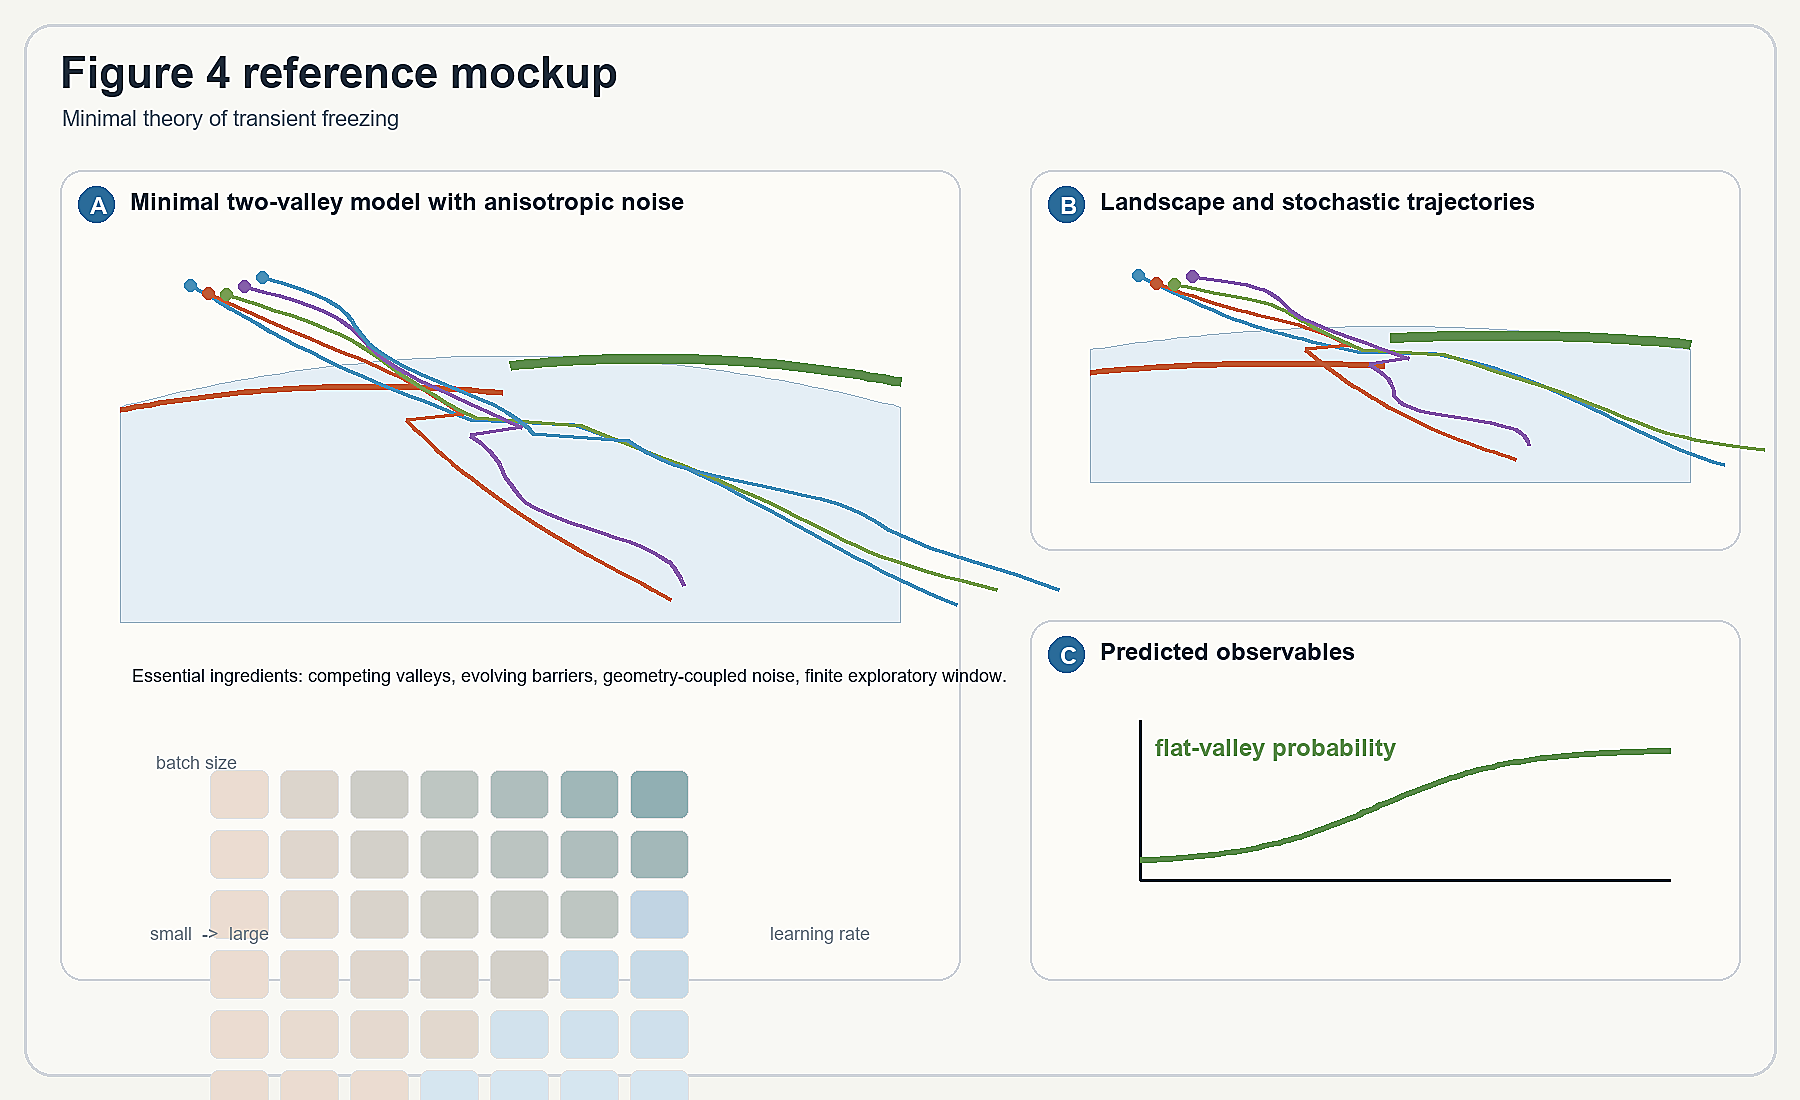
\includegraphics[width=\linewidth]{Figures_reference_mockups/FigRef4_minimal_model_mockup.png}
\caption{Minimal two-valley model. (A) The coordinate $y$ describes downhill training, while $x$ distinguishes a flat and a sharp valley. The valleys separate and the barrier grows as $y$ increases. (B) Geometry-coupled noise is stronger along high-curvature directions, mimicking the anisotropic structure of SGD noise. (C) Simulated trajectories hop between valleys early and freeze into one valley later. (D) The model predicts that stronger effective noise $\Delta_S$ increases both the freezing time and the final probability of selecting the flat valley.}
\label{fig:minimal_model}
\end{figure}

\subsection{Static Bias Is Real but Insufficient}
The reduced model also explains why a fixed-landscape theory is incomplete. At an approximately fixed $y$, the transverse coordinate $x$ can relax faster than the longitudinal drift. In this quasi-steady regime, anisotropic SGD noise generates a nonequilibrium preference for the flatter valley \cite{xieDiffusionTheoryDeep2021,zhuAnisotropicNoiseStochastic2019,yangStochasticGradientDescent2023}. Let $\delta f(y)\equiv f_{\mathrm{sharp}}(y)-f_{\mathrm{flat}}(y)$. Kramers-rate estimates give the flat-valley occupation probability
\begin{equation}
\begin{split}
P_{\mathrm{flat}}^{\mathrm{ss}}(y)
&\approx \left[1 + \gamma^{-\frac{1}{2}}
\exp\!\left(\frac{\Delta \mathcal{L}(y)\delta f(y)}{2\Delta_S}\right)\right]^{-1}.
\end{split}
\label{eq:steady_state_bias}
\end{equation}
Because $f_{\mathrm{flat}}>f_{\mathrm{sharp}}$, $\delta f<0$ and this expression is biased toward the broader valley. Equivalently, the anisotropic noise reshapes the effective landscape by lowering the flat valley relative to the sharp one.

However, Eq.~(\ref{eq:steady_state_bias}) also exposes the limitation of a static picture. If $y$ is held fixed, increasing $\Delta_S$ does not necessarily make the flat valley more selectively occupied. A larger effective noise level can mix the two valleys and weaken the instantaneous fixed-slice preference. This trend is opposite to the observed final outcome, where stronger SGD noise often leads to a higher probability of ending in flatter minima.

The resolution is that the final outcome is not a steady-state probability evaluated at an arbitrary fixed $y$. The landscape evolves while the escape rates collapse. The probability that matters is the quasi-steady bias at the last point where inter-valley hopping remains effective. Stronger noise can therefore reduce the fixed-slice selectivity and still enhance final flat-minimum selection, because it moves the freezing point to a later part of the landscape.

This distinction is the core of the transient-freezing mechanism. Static bias determines the direction of selection on a given landscape slice. Freezing determines which slice is inherited as the final basin choice. Both ingredients are needed to explain why noise promotes flat minima during real training.

\begin{figure}[!tbp]
\centering
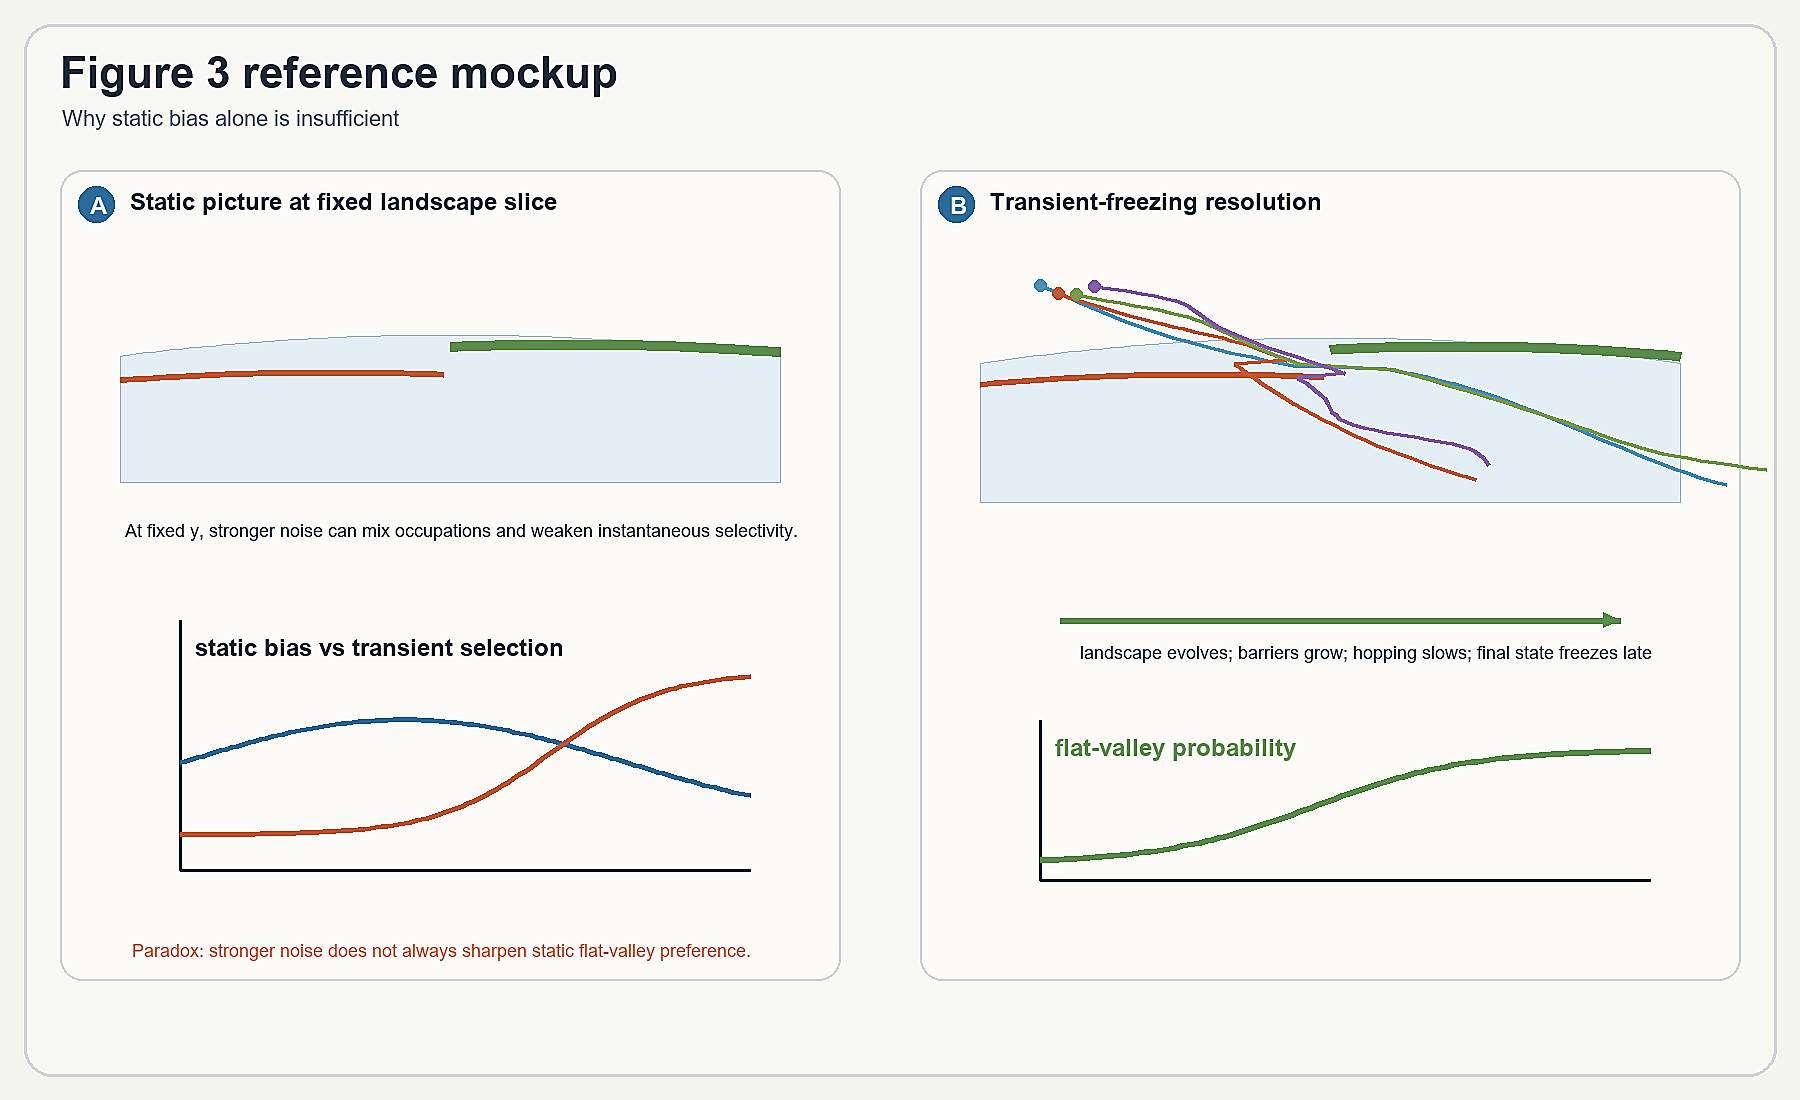
\includegraphics[width=\linewidth]{Figures_reference_mockups/FigRef3_static_bias_mockup.png}
\caption{Static bias and its limitation. (A) On a fixed landscape slice, anisotropic noise induces an effective loss that favors the flatter valley. (B) The corresponding quasi-steady flat-valley probability $P_{\mathrm{flat}}^{\mathrm{ss}}(y)$ is larger than the equilibrium expectation. (C) At fixed $y$, increasing $\Delta_S$ can reduce instantaneous selectivity by mixing the two valleys. (D) The apparent contradiction is resolved by recognizing that stronger noise delays freezing, so the final probability is inherited from a later landscape slice.}
\label{fig:static_bias}
\end{figure}

\section{Quantitative Predictions and Experimental Tests}
The theory becomes predictive when the final occupation is written as a stopping-time quantity. Let $y_f$ be the training coordinate at which inter-valley hopping becomes negligible. Then
\begin{equation}
P_{\mathrm{flat}}^{\mathrm{tr}} \approx P_{\mathrm{flat}}^{\mathrm{ss}}\!\left(y_f\right).
\label{eq:transient_selection}
\end{equation}
This expression does not assume that training reaches a global steady state. It assumes only that, before freezing, the transverse valley coordinate relaxes faster than the downhill coordinate, so the last quasi-steady bias is inherited by the final basin.

The freezing coordinate is determined by a competition of time scales. The inter-valley escape time is $\tau_{\mathrm{esc}}\sim(k_{f\to s}+k_{s\to f})^{-1}$, whereas the landscape changes on a drift time $\tau_y\sim |\dot y|^{-1}$. Freezing occurs when $\tau_{\mathrm{esc}}$ becomes longer than the time over which the quasi-steady distribution changes appreciably. In the two-valley model this criterion gives, up to slowly varying prefactors,
\begin{equation}
 y_f \approx y_b\,
 \frac{\sqrt{\Delta_S\ln\left(\Delta_S/\varepsilon^2\Phi^2\right)}}
 {x_2-\sqrt{\Delta_S\ln\left(\Delta_S/\varepsilon^2\Phi^2\right)}},
\label{eq:y_freeze}
\end{equation}
where $\varepsilon$ defines the arrest criterion and $\Phi$ collects model parameters that vary slowly compared with the escape rates. The important consequence is monotonic: larger $\Delta_S$ pushes the freezing point to larger $y$ over the relevant range.

Substituting this freezing point into Eq.~(\ref{eq:transient_selection}) yields a final flat-valley probability that increases with $\Delta_S$ for $\gamma>1$,
\begin{equation}
P_{\mathrm{flat}}^{\mathrm{tr}}
\approx \left[1+\gamma^{-\frac{1}{2}}
\left(\frac{\sqrt{\Delta_S}}{\varepsilon\Phi}\right)^{1-\gamma}\right]^{-1}.
\label{eq:final_selection}
\end{equation}
Thus the model predicts the empirical trend that stronger noise promotes flat-minimum selection, even though the fixed-slice selectivity alone would suggest the opposite.

The framework makes three direct predictions. First, increasing SGD noise increases the freezing time over the stable training range. Second, later freezing enlarges the accessible set of final solutions and shifts that set toward flatter endpoints. Third, different optimizers or schedules become comparable when they generate the same ordering of time scales: early inter-valley relaxation followed by barrier-driven arrest. These predictions can be tested by comparing freezing time, final-solution spread, flatness, and flat-valley probability across learning rates and batch sizes.

\begin{figure*}[!tbp]
\centering
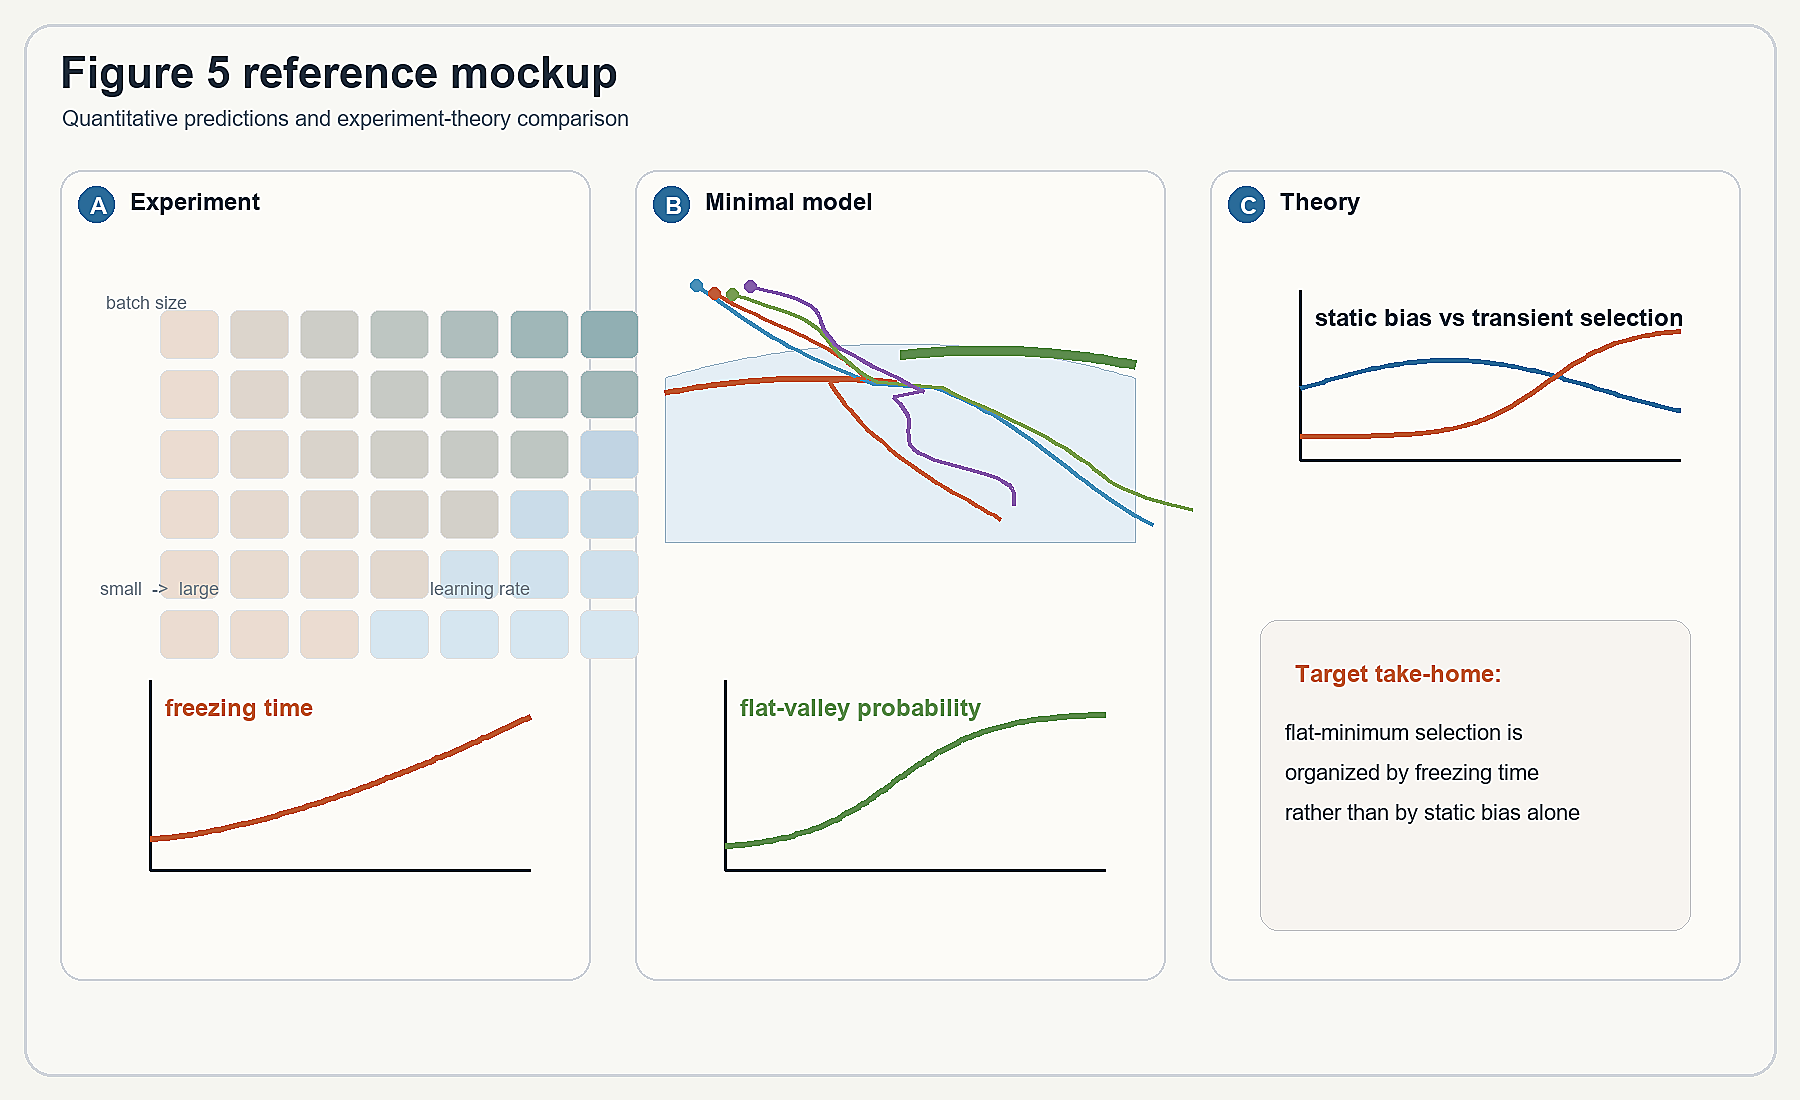
\includegraphics[width=0.98\textwidth]{Figures_reference_mockups/FigRef5_predictions_mockup.png}
\caption{Predictions and experiment-theory comparison. (A) The transient theory predicts that stronger effective noise delays freezing. (B) Evaluating the quasi-steady flat-valley bias at the freezing point predicts an increasing final flat-valley probability with noise. (C) Minimal-model simulations test the predicted relation between $\Delta_S$, $t_f$, and $P_{\mathrm{flat}}$. (D) Neural-network data are organized by the same variables: final-solution spread, final flatness, and upper-envelope test performance are compared with the measured freezing time. This comparison tests whether $t_f$ is the stopping-time variable that organizes the inherited final-solution ensemble.}
\label{fig:predictions}
\end{figure*}

\section{Discussion}
We have shown that flat-minimum selection in SGD can be viewed as a nonequilibrium freezing problem. The central mechanism is that SGD first remains mobile among competing valleys and then becomes committed when inter-valley motion stops. The final basin is therefore selected at a finite stopping time, not only by a late-time steady state inside an already chosen valley.

This perspective clarifies the role of noise. SGD noise is not merely a scalar regularizer that always increases an instantaneous preference for flatness. Its main role is dynamical: it controls the duration of the exploratory window before basin commitment. Stronger noise can keep the trajectory mobile until later in training, where the evolving landscape and the geometry-induced bias together make selection of the flatter valley more likely.

The mechanism also gives a design principle. Learning-rate and batch-size schedules should be understood as tools for controlling the timing of basin commitment, not only as tools for guaranteeing convergence. A schedule that preserves inter-valley mobility too briefly may freeze into a sharp basin; a schedule that preserves it too long may prevent reliable convergence. The useful objective is to regulate the freezing time so that exploration persists until favorable valleys are accessible and then arrests before late-time noise destroys refinement.

The model is deliberately minimal, so its scope conditions are explicit. The transient-freezing picture should apply when there are multiple competing valleys, geometry-coupled stochasticity, barriers that evolve during descent, and a finite time window in which valley exchange is possible. These ingredients are not specific to the small network used here and are expected in richer architectures and datasets. What may change across systems is the most informative continuation protocol, endpoint-similarity measure, and dimensionality of the effective valley-coordinate space.

More broadly, the results connect the implicit bias of SGD to a class of nonequilibrium selection problems in which the outcome depends on the pathway to arrest. Fixed-landscape effective potentials remain useful because they determine the local direction of the bias. They become predictive of the final solution only when combined with the freezing time at which that bias is locked in. From this viewpoint, SGD selects flat minima not simply because they are statically favored, but because noise delays the freezing point at which basin competition is resolved.

\section*{Data and Code Availability}
The code used for the empirical experiments and the two-valley simulations is available at
\url{https://github.com/YangNing1995/Transient_Dynamics_SGD}.

\begin{acknowledgments}
The work by N.Y. and C.T. was supported by the National Natural Science Foundation of China (Grant No. 12505089) and Fundamental and Interdisciplinary Disciplines Breakthrough Plan of the Ministry of Education of China (JYB2025XDXM502). The Flatiron Institute is a division of the Simons Foundation.
\end{acknowledgments}

\bibliography{deeplearning}

\end{document}
